% Options for packages loaded elsewhere
\PassOptionsToPackage{unicode}{hyperref}
\PassOptionsToPackage{hyphens}{url}
\documentclass[UTF8,a4paper,12pt]{ctexart}
\usepackage{xcolor}
\usepackage{amsmath,amssymb}
\setcounter{secnumdepth}{-\maxdimen} % remove section numbering
\usepackage{iftex}
\ifPDFTeX
  \usepackage[T1]{fontenc}
  \usepackage[utf8]{inputenc}
  \usepackage{textcomp} % provide euro and other symbols
\else % if luatex or xetex
  \usepackage{unicode-math} % this also loads fontspec
  \defaultfontfeatures{Scale=MatchLowercase}
  \defaultfontfeatures[\rmfamily]{Ligatures=TeX,Scale=1}
\fi
\usepackage{lmodern}
\ifPDFTeX\else
  % xetex/luatex font selection
\fi
% Use upquote if available, for straight quotes in verbatim environments
\IfFileExists{upquote.sty}{\usepackage{upquote}}{}
\IfFileExists{microtype.sty}{% use microtype if available
  \usepackage[]{microtype}
  \UseMicrotypeSet[protrusion]{basicmath} % disable protrusion for tt fonts
}{}
\makeatletter
\@ifundefined{KOMAClassName}{% if non-KOMA class
  \IfFileExists{parskip.sty}{%
    \usepackage{parskip}
  }{% else
    \setlength{\parindent}{0pt}
    \setlength{\parskip}{6pt plus 2pt minus 1pt}}
}{% if KOMA class
  \KOMAoptions{parskip=half}}
\makeatother
\usepackage{graphicx}
\makeatletter
\newsavebox\pandoc@box
\newcommand*\pandocbounded[1]{% scales image to fit in text height/width
  \sbox\pandoc@box{#1}%
  \Gscale@div\@tempa{\textheight}{\dimexpr\ht\pandoc@box+\dp\pandoc@box\relax}%
  \Gscale@div\@tempb{\linewidth}{\wd\pandoc@box}%
  \ifdim\@tempb\p@<\@tempa\p@\let\@tempa\@tempb\fi% select the smaller of both
  \ifdim\@tempa\p@<\p@\scalebox{\@tempa}{\usebox\pandoc@box}%
  \else\usebox{\pandoc@box}%
  \fi%
}
% Set default figure placement to htbp
\def\fps@figure{htbp}
\makeatother
\ifLuaTeX
\usepackage[bidi=basic,shorthands=off,,provide=*]{babel}
\else
\usepackage[bidi=default,shorthands=off,,provide=*]{babel}
\fi
\ifLuaTeX
  \usepackage{selnolig} % disable illegal ligatures
\fi
\setlength{\emergencystretch}{3em} % prevent overfull lines
\providecommand{\tightlist}{%
  \setlength{\itemsep}{0pt}\setlength{\parskip}{0pt}}
\usepackage[a4paper,margin=2.5cm]{geometry}
\setCJKmainfont{SimSun}
\setCJKsansfont{SimHei}
\usepackage{newunicodechar}
\newunicodechar{γ}{\ensuremath{\gamma}}
\newunicodechar{µ}{\textmu}
\usepackage{graphicx}
\usepackage{float}
\usepackage{caption}
\usepackage{setspace}
\usepackage{titlesec}
\usepackage{fancyhdr}
\usepackage{lastpage}
\usepackage{hyperref}
\hypersetup{colorlinks=true,linkcolor=black,urlcolor=blue,citecolor=black,pdftitle={^60Co γ 射线 0–60 krad(Si) 累积辐照下 S、T 组器件电学特性分析}}
\setlength{\parindent}{2em}
\setlength{\parskip}{0.35em}
\linespread{1.25}\selectfont
\setkeys{Gin}{width=0.88\linewidth,keepaspectratio}
\captionsetup{font=small,labelfont=bf,labelsep=space,skip=6pt}
\titleformat{\section}{\Large\bfseries}{\thesection}{0.75em}{}
\titleformat{\subsection}{\large\bfseries}{\thesubsection}{0.75em}{}
\titleformat{\subsubsection}{\normalsize\bfseries}{\thesubsubsection}{0.75em}{}
\pagestyle{fancy}
\fancyhf{}
\fancyfoot[C]{\thepage\ / \pageref{LastPage}}
\renewcommand{\headrulewidth}{0pt}
\usepackage{bookmark}
\IfFileExists{xurl.sty}{\usepackage{xurl}}{} % add URL line breaks if available
\urlstyle{same}
\hypersetup{
  pdftitle={\^{}60Co γ 射线 0--60 krad(Si) 累积辐照下 S、T 组器件电学特性分析},
  pdflang={zh-CN},
  hidelinks,
  pdfcreator={LaTeX via pandoc}}

\title{\^{}60Co γ 射线 0--60 krad(Si) 累积辐照下 S、T
组器件电学特性分析}
\author{}
\date{}

\begin{document}
\maketitle

\section{摘要}\label{ux6458ux8981}

本报告分析两组样品器件在 \^{}60Co γ 射线累积总电离剂量为
0、10、20、30、40、50 和 60 krad(Si) 时的电学响应。每个剂量增量为 10
krad(Si)，照射时间为 198 s；辐照期间施加 20 V
偏置并设置适当限流保护，实验在室温环境下进行。S1--S3 与 T1--T3
分别为跨剂量持续跟踪的同一批器件，每组 n=3。转移特性在固定漏源电压
\(V_{DS}=0.1\) V 下测量，输出特性在固定栅源电压 \(V_{GS}=-20\)
V、\(V_{DS}=0\)--150 V 下测量。由于原始 Excel 中 GM、VT 列含
\texttt{\#REF}，本分析仅依据 DrainI--GateV
原始列统一重算峰值跨导、切线外推阈值电压和亚阈值摆幅；输出分析以
10、20、30 V 的共同安全偏压及达到指定漏电流的电压为主，避免将约 10 mA
合规限流区误作剂量响应。

数据直接显示，两组器件均发生随累积剂量增加而持续扩大的负向阈值漂移和峰值跨导下降。60
krad(Si) 时，S 组阈值漂移为 \(-6.120\pm0.045\) V，峰值跨导相对基线下降
\((60.25\pm1.96)\%\)；T 组对应值为 \(-9.969\pm0.337\) V 和
\((61.21\pm4.10)\%\)。亚阈值摆幅由 S 组的 \(188.3\pm1.0\) mV/dec 增至
\(321.9\pm30.7\) mV/dec，而 T 组由 \(225.4\pm2.8\) mV/dec 增至
\(1674.0\pm35.4\) mV/dec。30 V 漏电流在 60 krad(Si) 时相对基线平均增加
1840\%（S 组）和 60.2\%（T 组），但 S 组个体间离散和剂量非单调性明显。S
组 20--60 krad(Si) 的 13 次后续加压扫描中，30 V
漏电相对同器件同剂量首次扫描降低
70.65\%--96.19\%，构成可重复观察到的扫描历史相关恢复现象，但不能据此单独确定微观机制。综合而言，本数据支持``总剂量累积导致转移特性系统性退化，同时输出漏电响应呈现组别差别和测量历史依赖''的描述；氧化层俘获电荷、界面态以及场致电荷重分布或去俘获仅作为与文献一致的候选解释。

\textbf{关键词：} \^{}60Co γ
射线；总电离剂量；阈值电压；跨导；亚阈值摆幅；漏电流；连续加压扫描

\section{1.
实验条件与数据处理方法}\label{ux5b9eux9a8cux6761ux4ef6ux4e0eux6570ux636eux5904ux7406ux65b9ux6cd5}

\subsection{1.1
实验设计与数据边界}\label{ux5b9eux9a8cux8bbeux8ba1ux4e0eux6570ux636eux8fb9ux754c}

辐照剂量点为 0--60 krad(Si)，间隔 10 krad(Si)，每个剂量增量对应 198 s 的
\^{}60Co γ 射线照射。辐照期间器件施加 20 V
偏置，并采用适当限流保护；实验在室温环境下完成。S、T
仅表示样品组标签。器件结构、材料、几何尺寸、制造工艺及封装属于商业保密信息，不在本报告披露和讨论范围内，因此本文不将两组差异归因于任何特定结构或工艺。S1--S3、T1--T3
是纵向跟踪的物理器件，而不是各剂量重新抽取的独立样本。

转移特性固定 \(V_{DS}=0.1\) V。不同剂量采用了不同 \(V_{GS}\)
扫描范围：低剂量主要为 \(-10\)--8
V，较高剂量逐步向负电压扩展。因此，曲线整体位移和从各自扫描范围内提取的局部参数可以比较，但固定
\(V_{GS}\)
电流只有在该电压同时落入相应扫描范围时才具可比性。输出特性固定
\(V_{GS}=-20\) V，只有一条 \(V_{DS}=0\)--150 V
扫描，不是多栅压输出曲线族。

\begin{figure}
\centering
\pandocbounded{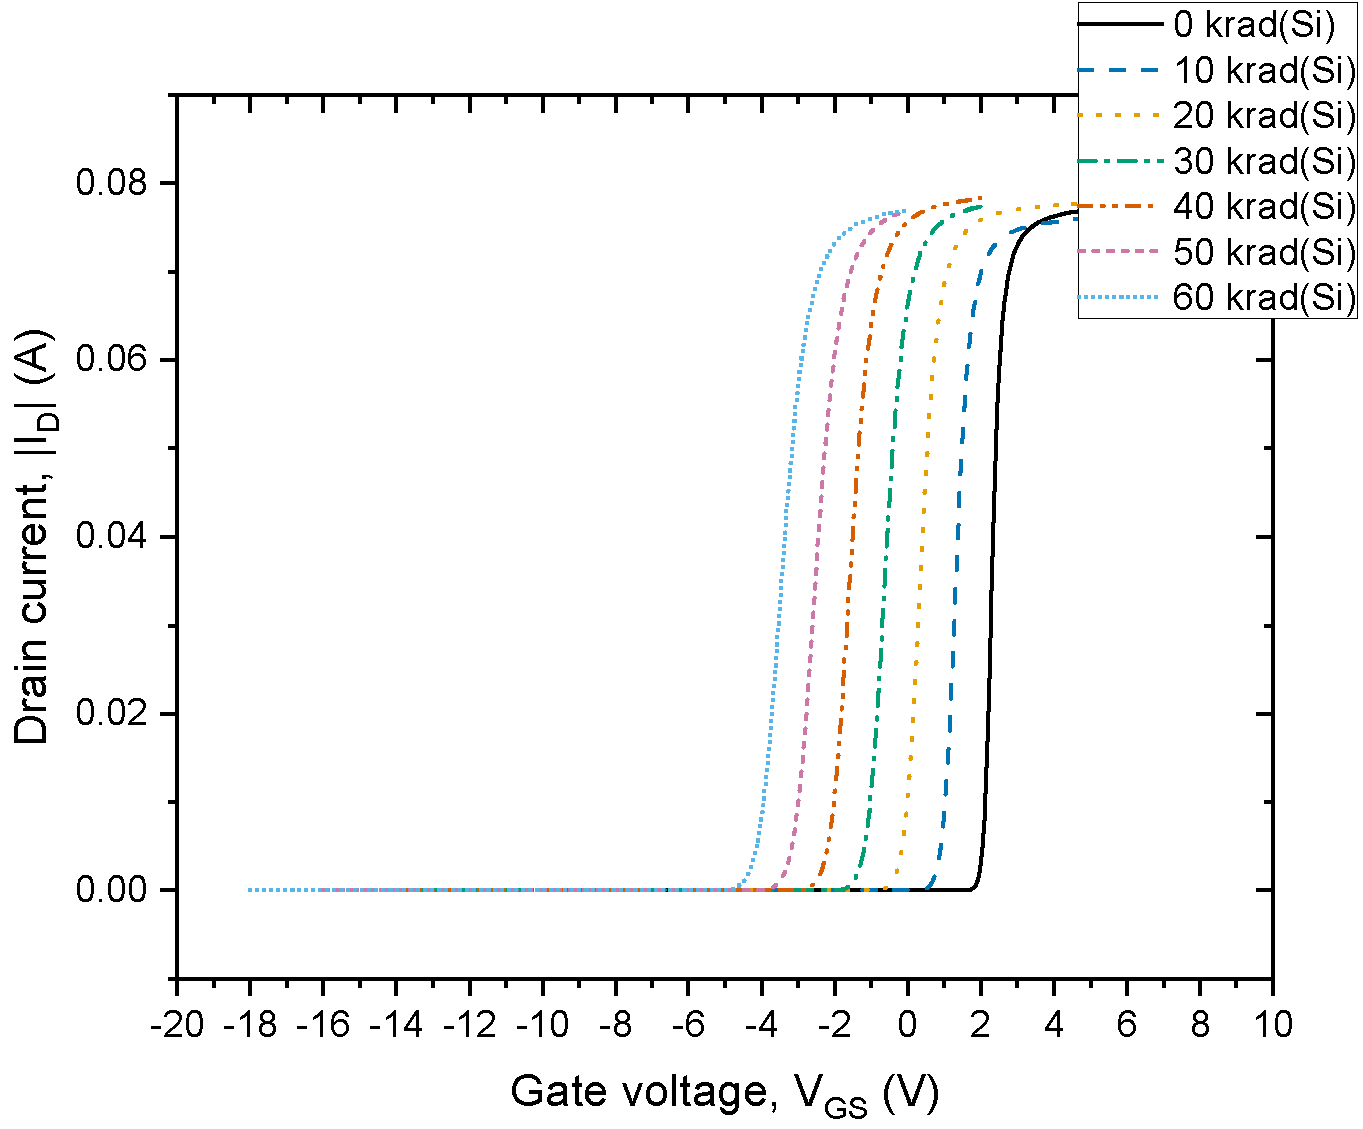
\includegraphics[keepaspectratio,alt={S组不同总剂量下的转移特性（线性坐标）}]{../03_figures/pdf/transfer_linear_S.pdf}}
\caption{S组不同总剂量下的转移特性（线性坐标）}
\end{figure}

\begin{figure}
\centering
\pandocbounded{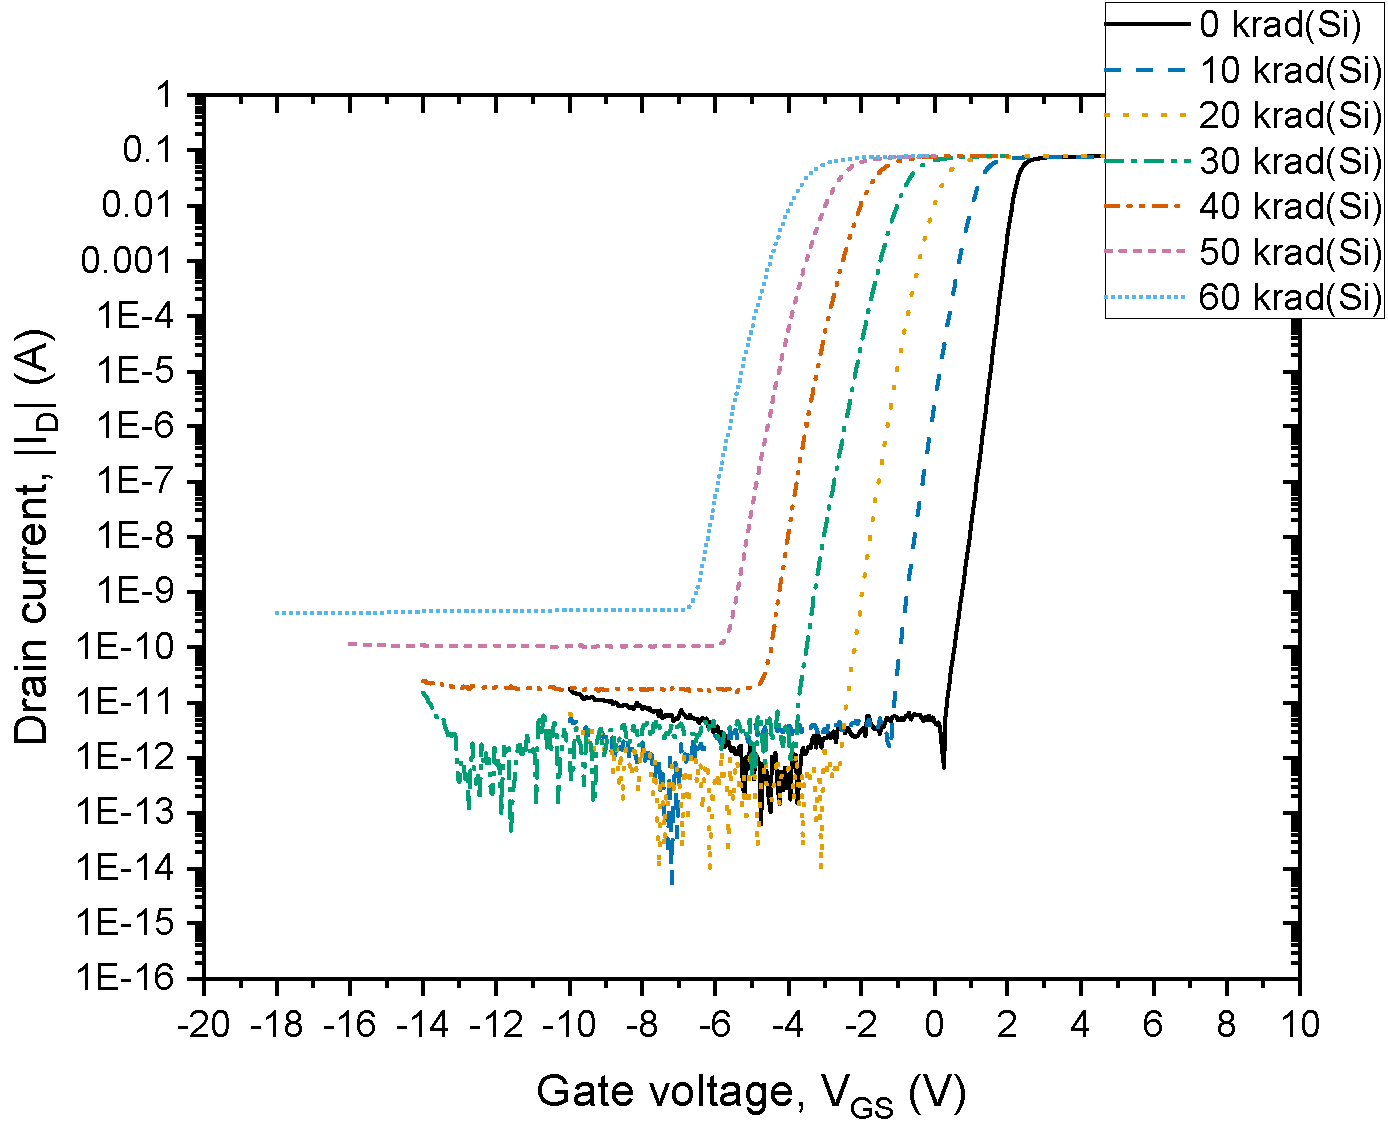
\includegraphics[keepaspectratio,alt={S组不同总剂量下的转移特性（半对数坐标）}]{../03_figures/pdf/transfer_semilog_S.pdf}}
\caption{S组不同总剂量下的转移特性（半对数坐标）}
\end{figure}

\begin{figure}
\centering
\pandocbounded{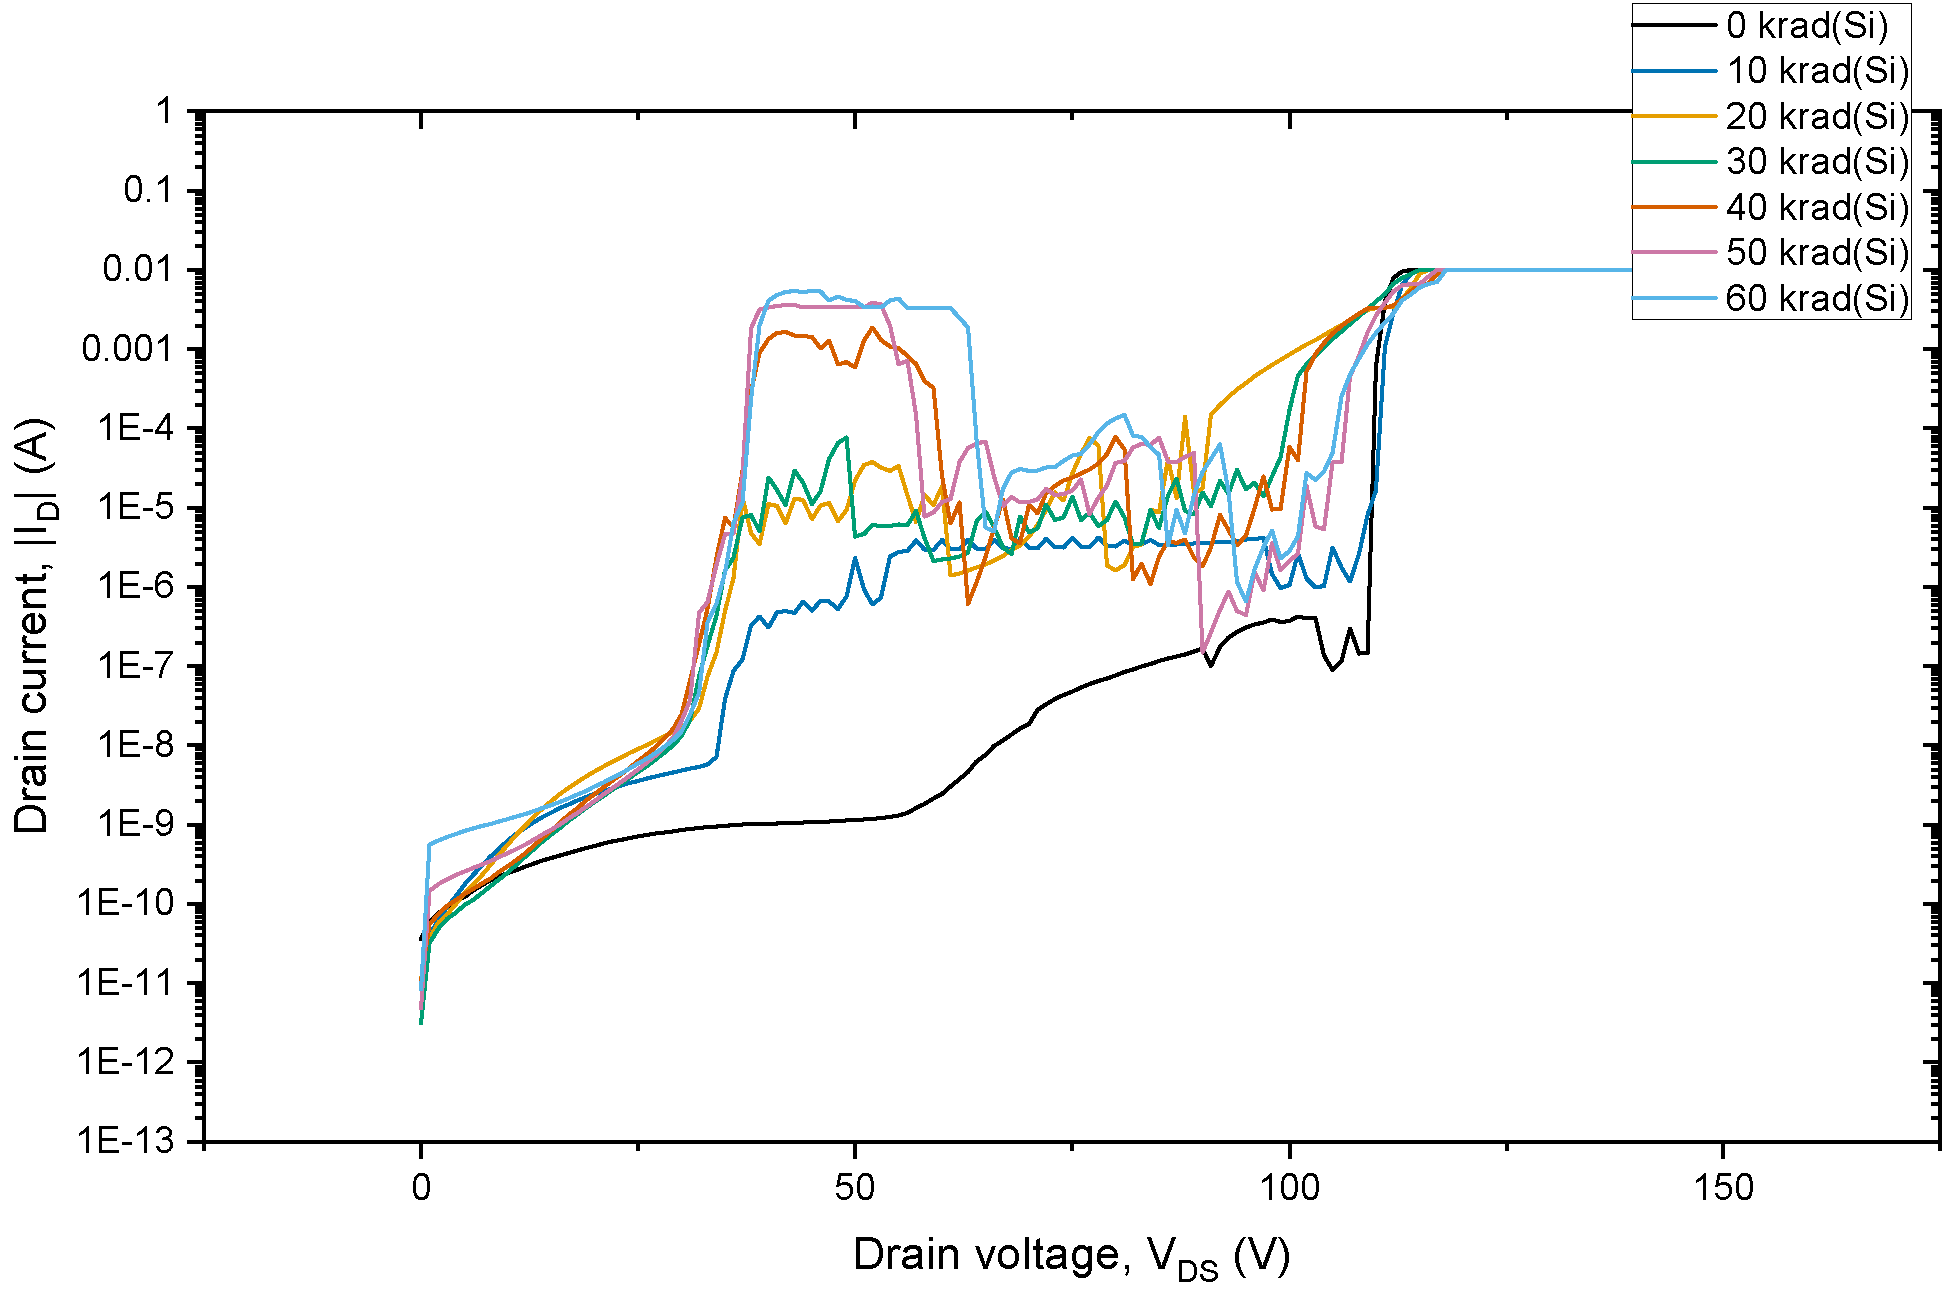
\includegraphics[keepaspectratio,alt={S组不同总剂量下的输出特性（VGS=-20 V，半对数坐标）}]{../03_figures/pdf/output_semilog_S.pdf}}
\caption{S组不同总剂量下的输出特性（VGS=-20 V，半对数坐标）}
\end{figure}

\begin{figure}
\centering
\pandocbounded{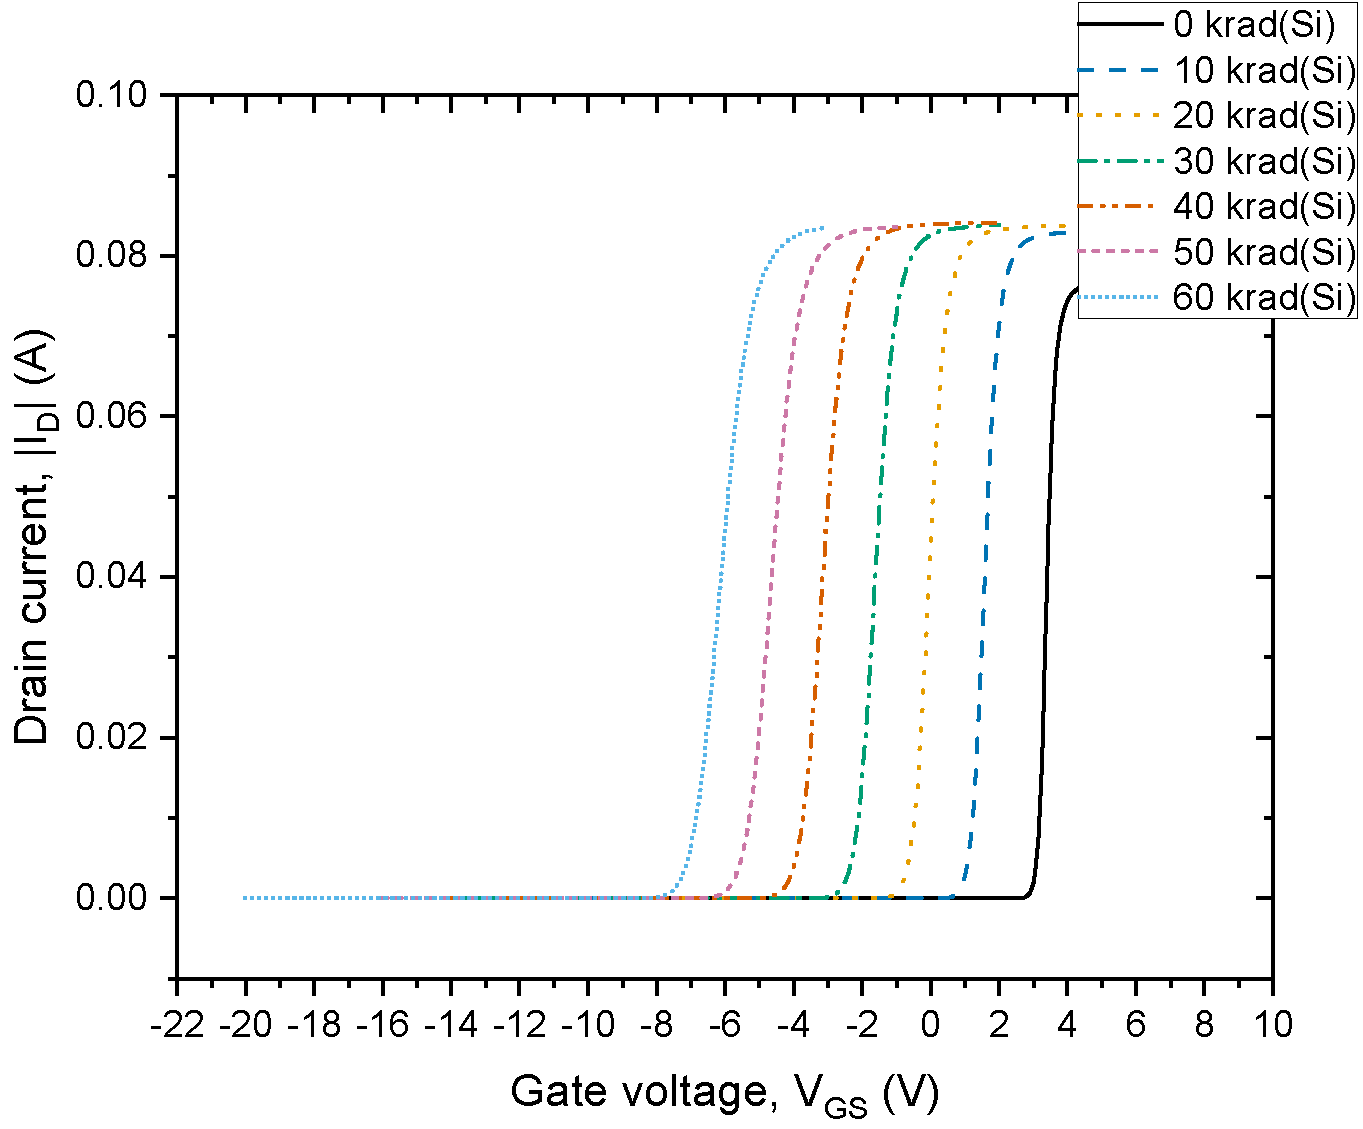
\includegraphics[keepaspectratio,alt={T组不同总剂量下的转移特性（线性坐标）}]{../03_figures/pdf/transfer_linear_T.pdf}}
\caption{T组不同总剂量下的转移特性（线性坐标）}
\end{figure}

\begin{figure}
\centering
\pandocbounded{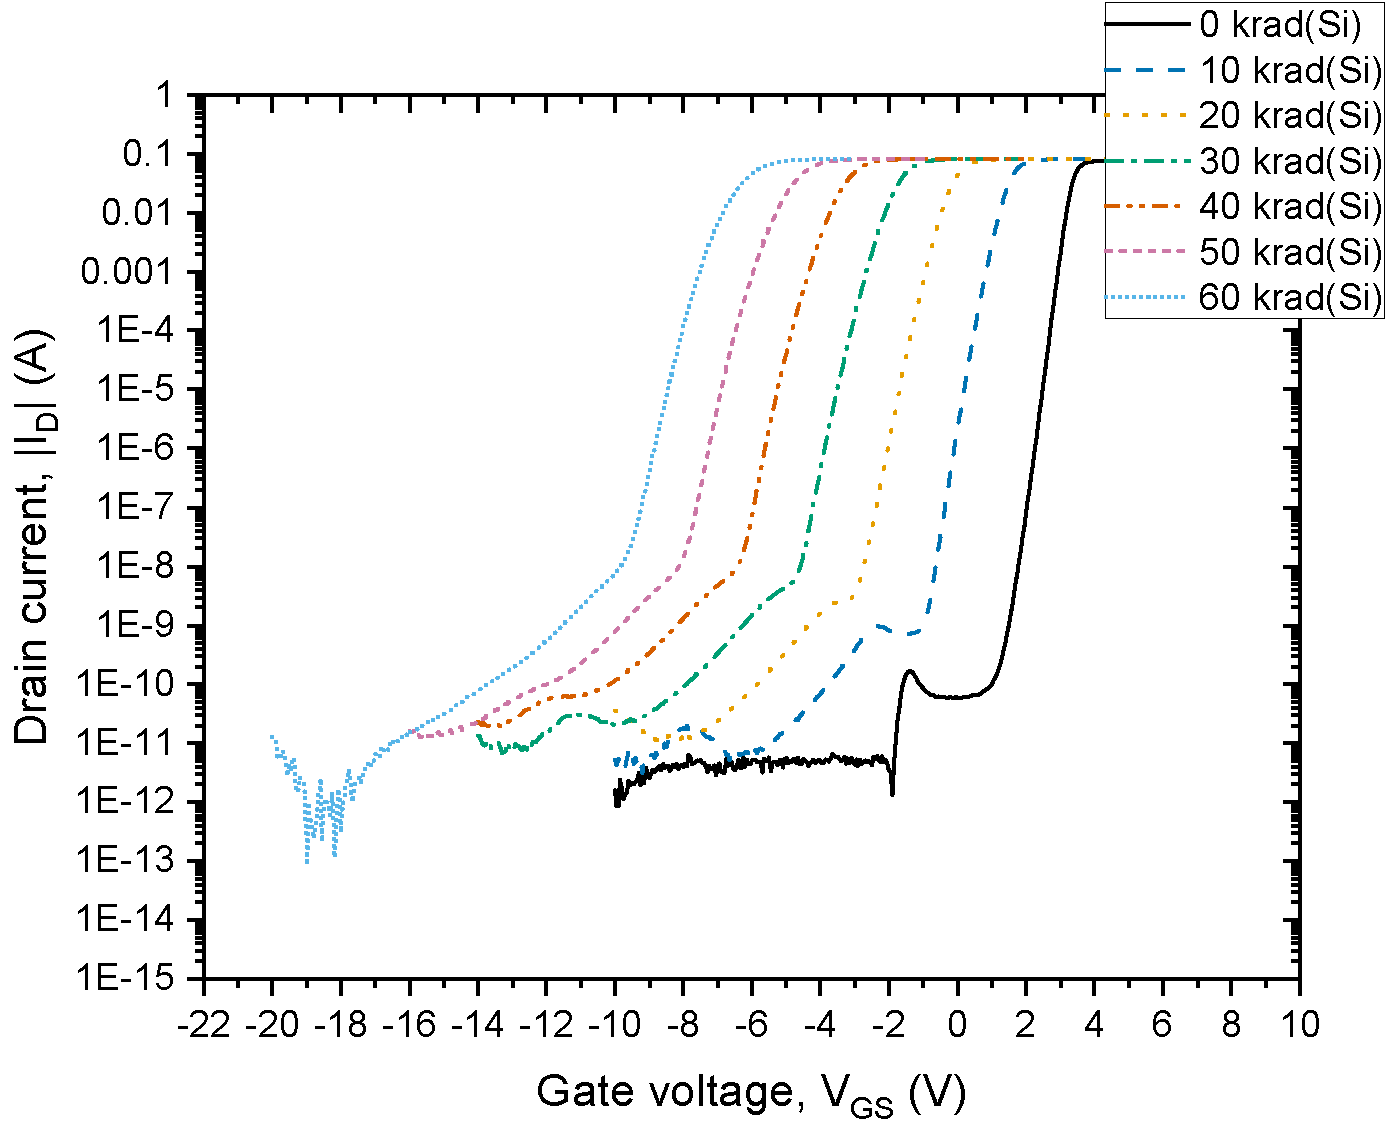
\includegraphics[keepaspectratio,alt={T组不同总剂量下的转移特性（半对数坐标）}]{../03_figures/pdf/transfer_semilog_T.pdf}}
\caption{T组不同总剂量下的转移特性（半对数坐标）}
\end{figure}

\begin{figure}
\centering
\pandocbounded{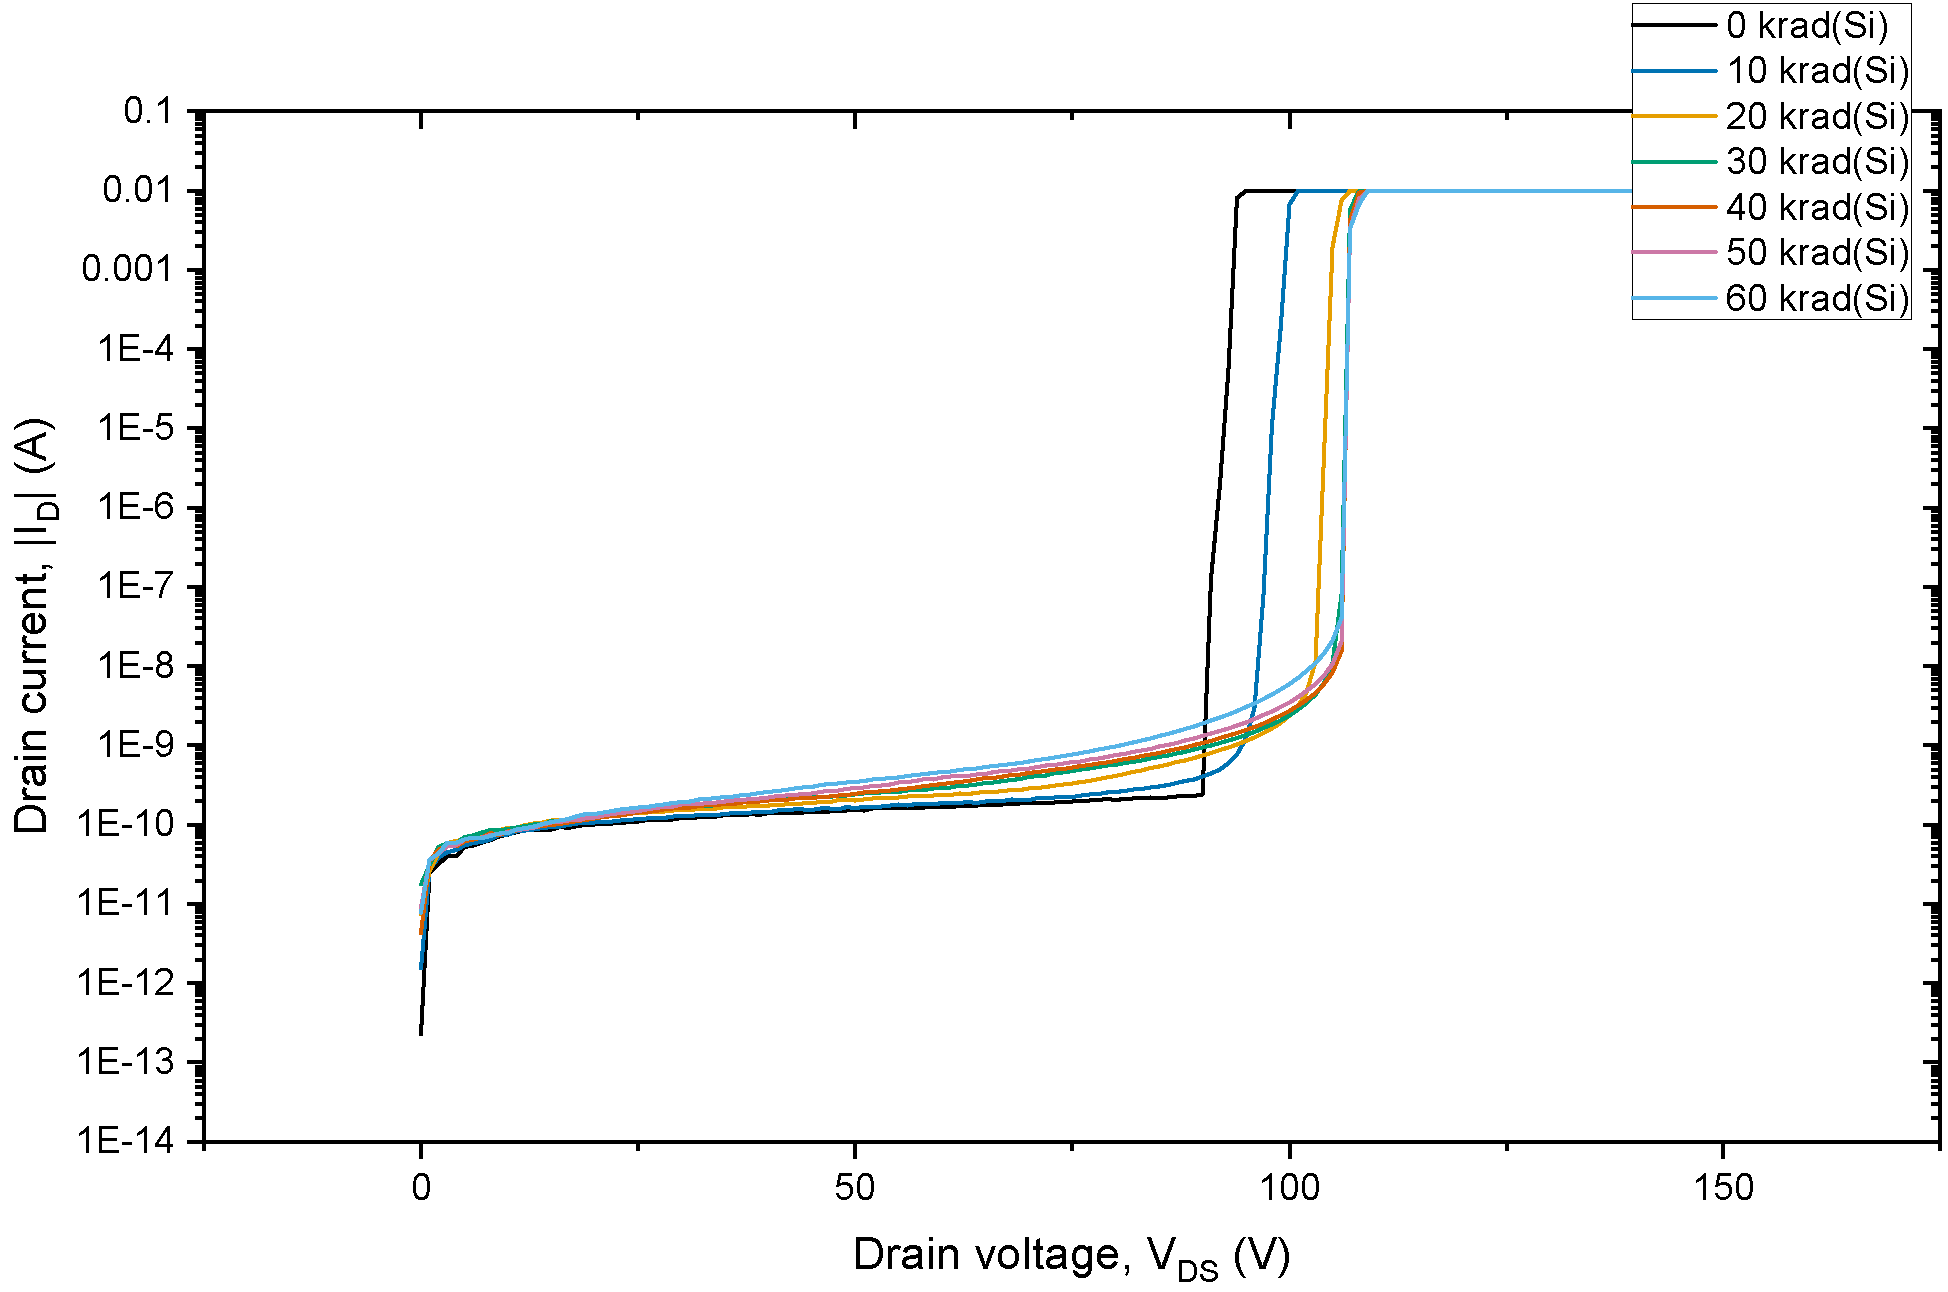
\includegraphics[keepaspectratio,alt={T组不同总剂量下的输出特性（VGS=-20 V，半对数坐标）}]{../03_figures/pdf/output_semilog_T.pdf}}
\caption{T组不同总剂量下的输出特性（VGS=-20 V，半对数坐标）}
\end{figure}

\subsection{1.2
参数重算与统计口径}\label{ux53c2ux6570ux91cdux7b97ux4e0eux7edfux8ba1ux53e3ux5f84}

原始 Excel 的 GM、VT 列共含 42
个错误标记，未直接进入正式分析。漏极电流先经 11 点、二阶 Savitzky--Golay
平滑，再对 \(V_{GS}\)
求数值梯度得到跨导；峰值跨导点的切线与电压轴交点定义为切线外推阈值电压。亚阈值摆幅由
\(\log_{10}|I_D|\) 对 \(V_{GS}\) 的 21 点滑动线性拟合得到，仅保留
\(R^2\ge0.98\) 的最佳窗口。各剂量变化均由同一器件相对其 0 krad(Si)
基线计算。

输出曲线在 10、20、30 V 处插值得到 \(|I_D|\) 和
\(|I_G|\)，并记录首次达到 \(1\ \mathrm{nA}\) 至 \(1\ \mathrm{mA}\)
的离散 \(V_{DS}\)。大量曲线在高压端达到约 10 mA 合规限流，故 150 V
电流不作为剂量指标。主汇总只纳入 \texttt{scan\_no=1}，每个组别和剂量均为
n=3；S 组的 \texttt{-2/-3/-4}
扫描只与同器件、同剂量首次扫描配对，不增加样本量。

统计结果以单器件轨迹、均值±样本标准差及相对 0 krad(Si)
的变化为主。对于跨数量级的漏电变化，另报告描述性效应量
\(\log_{10}(I_{60}/I_0)\)：0 表示无变化，1 表示增大一个数量级。每组仅
n=3，效应量只用于表述本批器件的变化幅度和一致性，不作显著性检验，也不报告
p 值。

\section{2.
转移特性随总剂量变化}\label{ux8f6cux79fbux7279ux6027ux968fux603bux5242ux91cfux53d8ux5316}

\subsection{2.1
阈值电压及其漂移}\label{ux9608ux503cux7535ux538bux53caux5176ux6f02ux79fb}

\textbf{数据直接显示：} 两组转移曲线均随剂量升高向负 \(V_{GS}\)
方向移动（图1、图2、图4、图5）。S 组平均阈值电压由 0 krad(Si) 时的
\(2.073\pm0.014\) V 依次变为 10、20、30、40、50、60 krad(Si) 时的
\(0.967\pm0.010\)、\(-0.079\pm0.011\)、\(-1.104\pm0.019\)、\(-2.106\pm0.024\)、\(-3.083\pm0.032\)
和 \(-4.047\pm0.035\) V。T 组由 \(3.143\pm0.032\) V 依次变为
\(1.205\pm0.068\)、\(-0.484\pm0.126\)、\(-2.121\pm0.183\)、\(-3.722\pm0.244\)、\(-5.284\pm0.297\)
和 \(-6.826\pm0.350\) V。

\begin{figure}
\centering
\pandocbounded{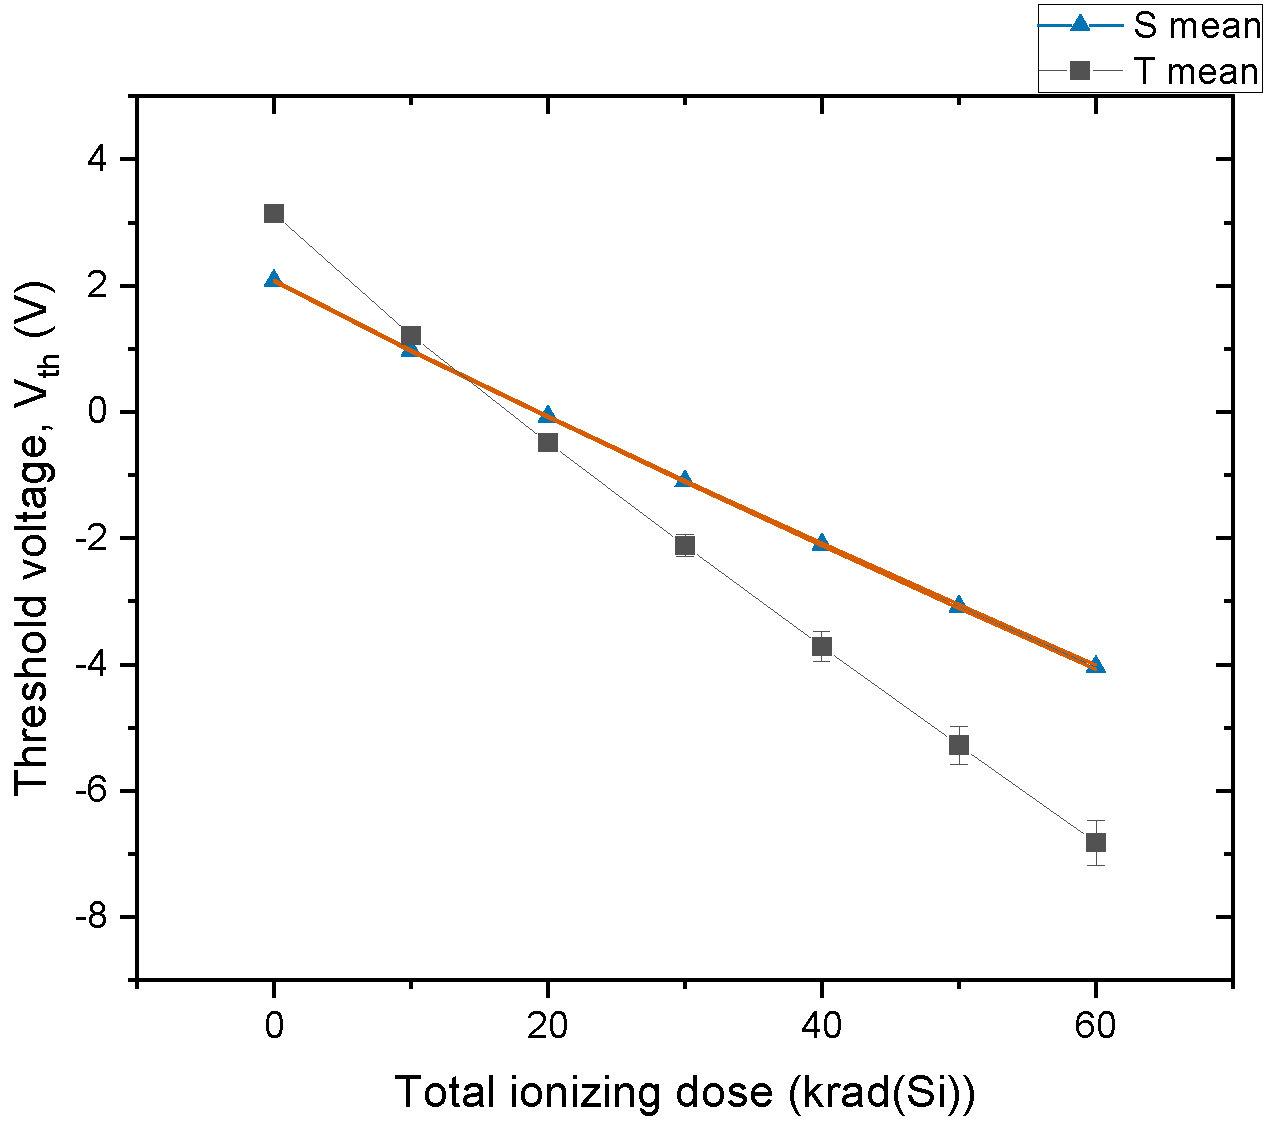
\includegraphics[keepaspectratio,alt={S/T组阈值电压随总剂量的变化}]{../03_figures/pdf/threshold_voltage.pdf}}
\caption{S/T组阈值电压随总剂量的变化}
\end{figure}

\begin{figure}
\centering
\pandocbounded{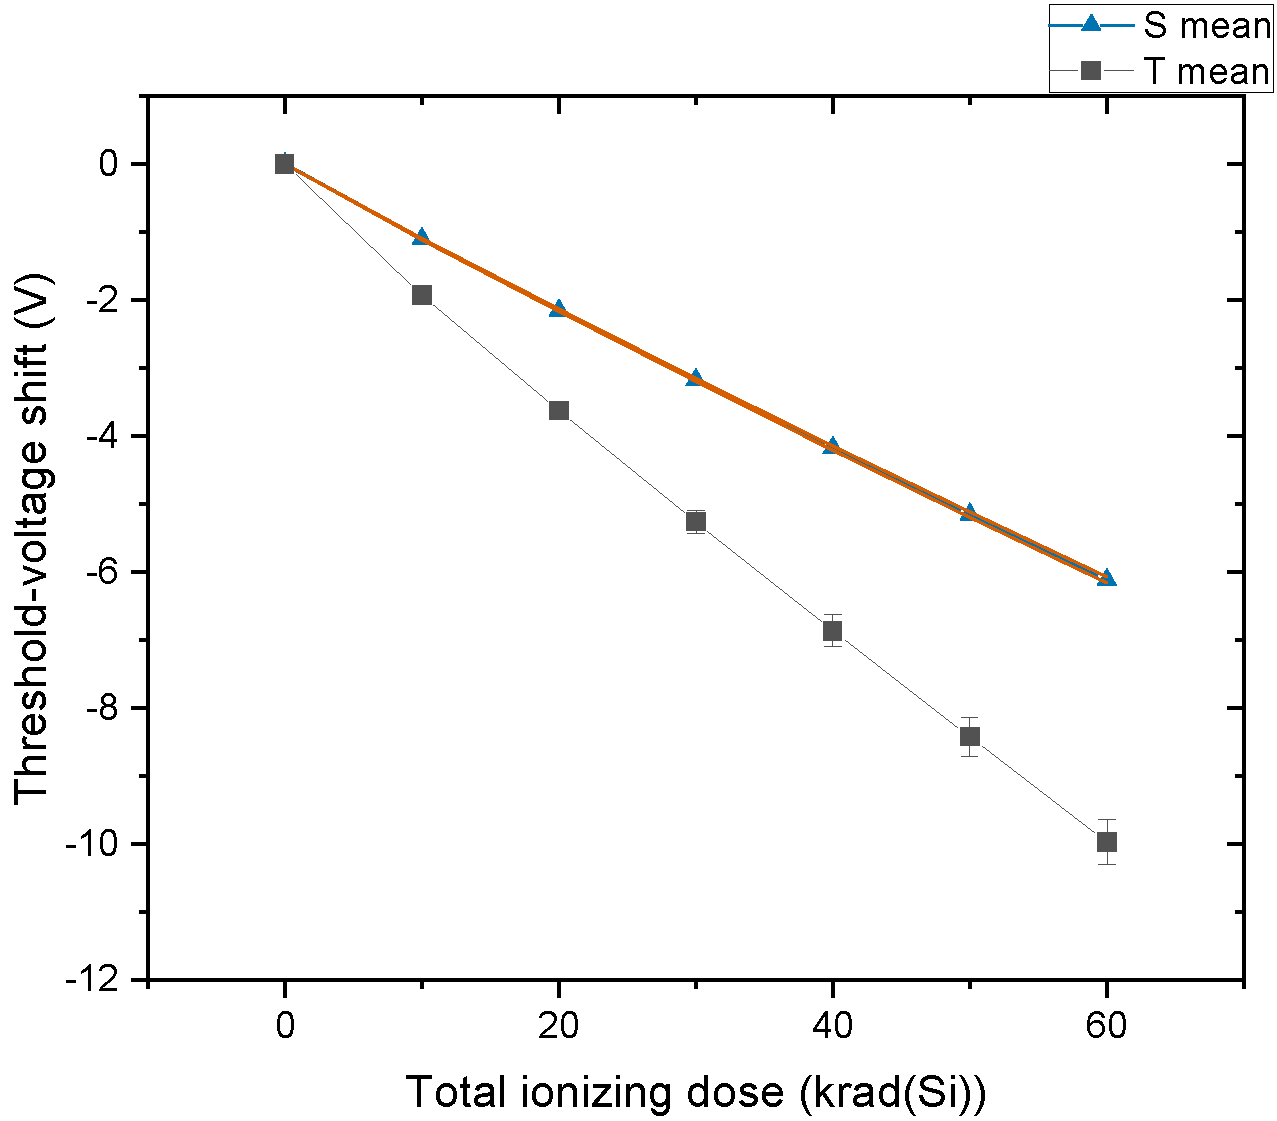
\includegraphics[keepaspectratio,alt={S/T组相对0 krad(Si)的阈值电压漂移}]{../03_figures/pdf/threshold_shift.pdf}}
\caption{S/T组相对0 krad(Si)的阈值电压漂移}
\end{figure}

\textbf{统计归纳：} 60 krad(Si) 时，S1--S3 的阈值变化分别为
\(-6.088\)、\(-6.172\)、\(-6.099\) V，组均值为 \(-6.120\pm0.045\)
V；T1--T3 分别为 \(-10.339\)、\(-9.885\)、\(-9.682\) V，组均值为
\(-9.969\pm0.337\) V。三条轨迹在各组内方向一致，但 n=3
不支持总体概率推断。就本批器件而言，T 组负向阈值漂移幅度大于 S
组；该差异不能外推至相应器件类别。

\subsection{2.2
峰值跨导与亚阈值摆幅}\label{ux5cf0ux503cux8de8ux5bfcux4e0eux4e9aux9608ux503cux6446ux5e45}

\textbf{数据直接显示：} S 组峰值跨导从 \(0.1481\pm0.0050\) S 降至
\(0.05883\pm0.00133\) S，60 krad(Si) 相对变化为 \(-(60.25\pm1.96)\%\)；T
组从 \(0.1500\pm0.0161\) S 降至 \(0.05777\pm0.00132\) S，相对变化为
\(-(61.21\pm4.10)\%\)（图9）。两组最终相对降幅接近，但 T 组在 10--30
krad(Si) 的器件间差异较大。

\begin{figure}
\centering
\pandocbounded{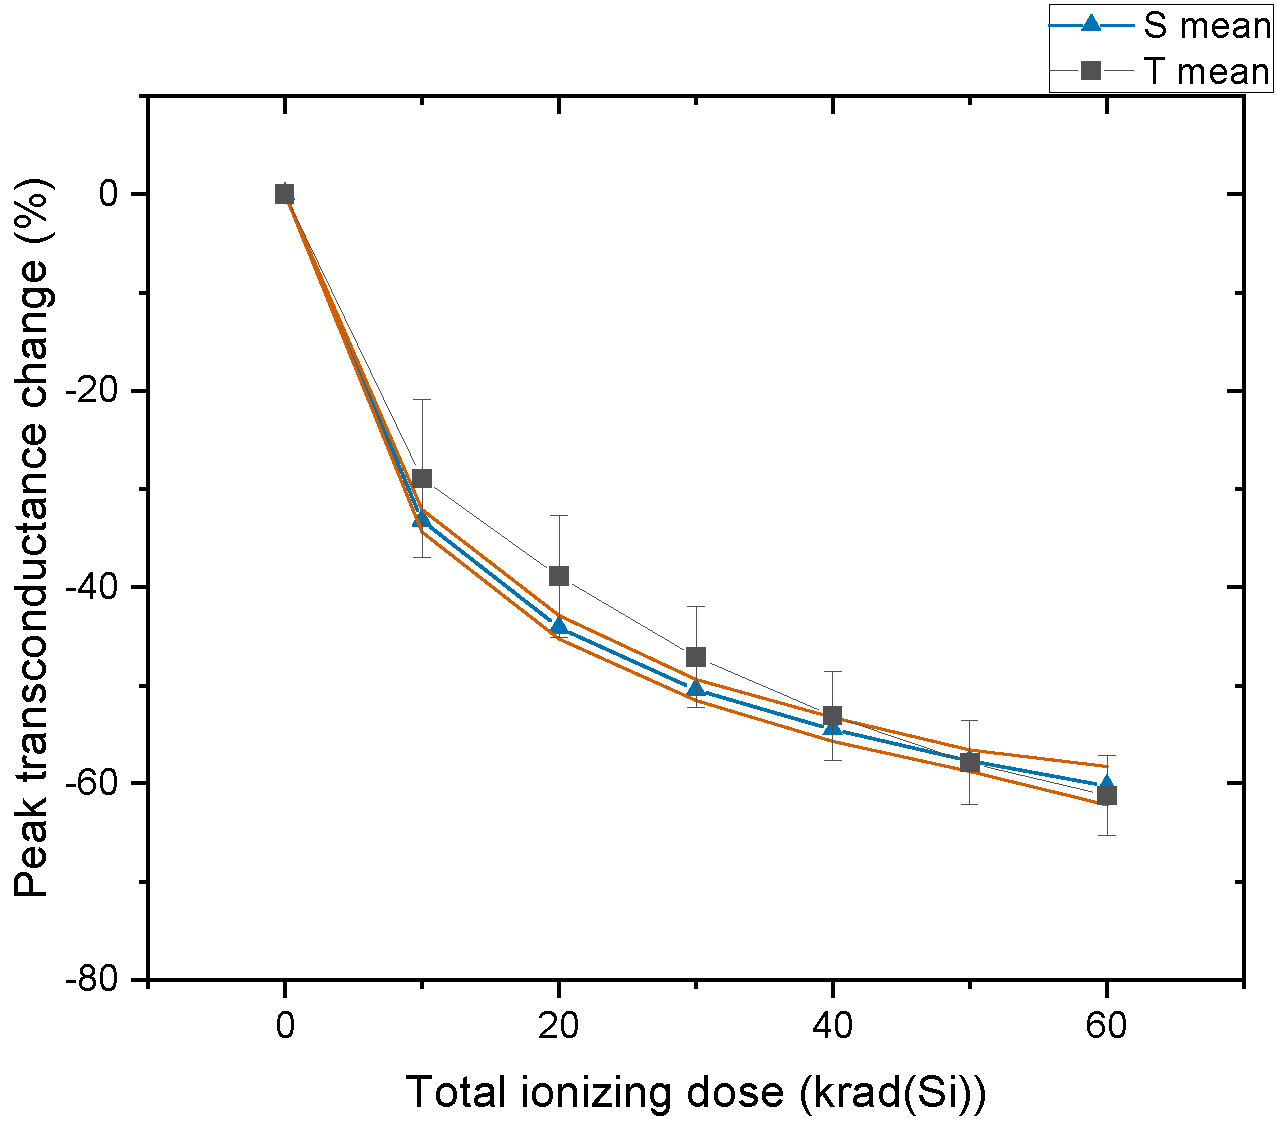
\includegraphics[keepaspectratio,alt={S/T组峰值跨导相对变化随总剂量的变化}]{../03_figures/pdf/gm_change.pdf}}
\caption{S/T组峰值跨导相对变化随总剂量的变化}
\end{figure}

亚阈值摆幅呈不同量级的恶化（图10）。S 组由 \(188.3\pm1.0\) mV/dec 增至
\(321.9\pm30.7\) mV/dec，配对增量为 \(133.6\pm31.7\) mV/dec。T 组由
\(225.4\pm2.8\) mV/dec 增至 \(1674.0\pm35.4\) mV/dec，配对增量为
\(1448.6\pm36.8\) mV/dec。T 组从 10 krad(Si) 起离散较大，10、20 krad(Si)
的标准差分别为 577.3 和 623.8 mV/dec；到 30--60
krad(Si)，三个器件均进入约 1515--1700 mV/dec 的高摆幅区间。

\begin{figure}
\centering
\pandocbounded{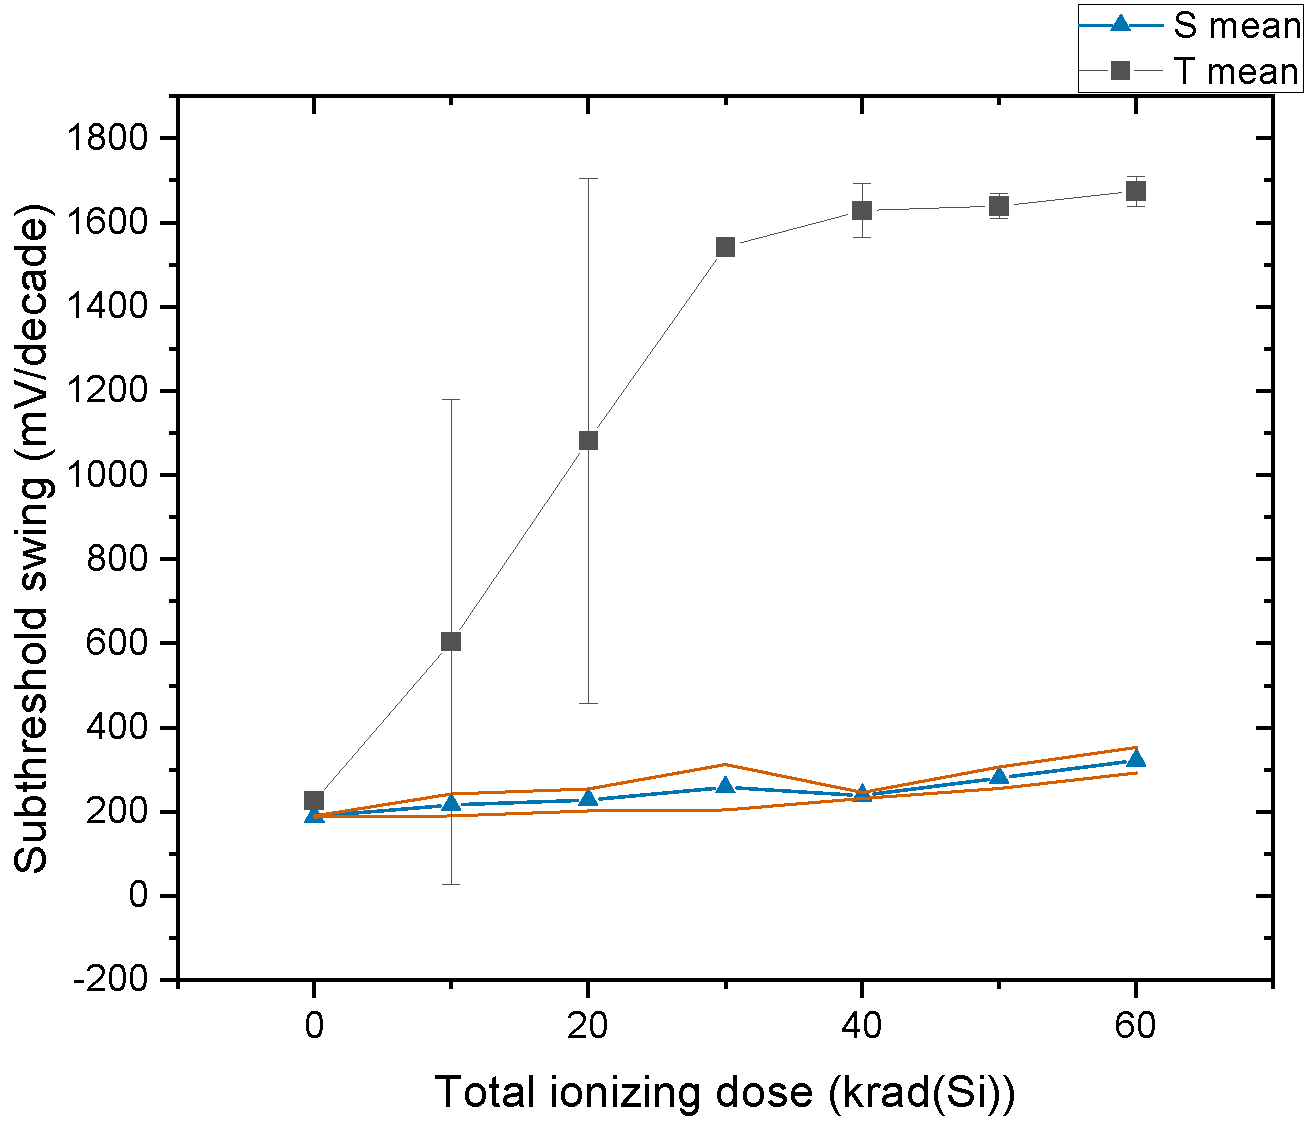
\includegraphics[keepaspectratio,alt={S/T组亚阈值摆幅随总剂量的变化}]{../03_figures/pdf/subthreshold_swing.pdf}}
\caption{S/T组亚阈值摆幅随总剂量的变化}
\end{figure}

\textbf{统计归纳：}
阈值漂移、跨导下降与亚阈值摆幅增大在每组的三条纵向轨迹中方向一致，说明它们不是由单个异常器件独立造成。但不同
\(V_{GS}\) 扫描范围、亚阈值窗口的自动选择以及 n=3
的限制，要求对摆幅绝对值的组间比较保持谨慎。

\section{3.
输出/漏电特性随总剂量变化}\label{ux8f93ux51faux6f0fux7535ux7279ux6027ux968fux603bux5242ux91cfux53d8ux5316}

\textbf{数据直接显示：} S 组 30 V 漏电均值由
\((8.66\pm3.37)\times10^{-10}\) A 增至 \((1.52\pm0.55)\times10^{-8}\)
A，60 krad(Si) 相对各器件基线的平均变化为 \(1840\%\pm992\%\)。三个器件的
60/0 krad(Si) 电流比分别约为 18.5、29.8 和 10.0 倍，对应
\(\log_{10}(I_{60}/I_0)=1.246\pm0.238\) decade。S
组变化并非严格单调：10--60 krad(Si) 的 30 V 均值依次约为
4.85、17.2、13.1、24.9、20.4 和 15.2 nA，且 10--20 krad(Si) 的离散主要受
S3 较大响应影响。

T 组 30 V 漏电由 \((1.219\pm0.034)\times10^{-10}\) A 增至
\((1.950\pm0.120)\times10^{-10}\) A，60 krad(Si) 相对基线变化为
\(60.2\%\pm11.9\%\)；三个器件的电流比为 1.73、1.59 和 1.49，对应
\(\log_{10}(I_{60}/I_0)=0.204\pm0.032\) decade。因此，图11所示的 S
组低压漏电增幅和离散均大于 T 组，但该比较仅适用于本批样品及固定
\(V_{GS}=-20\) V 的测试条件。

\begin{figure}
\centering
\pandocbounded{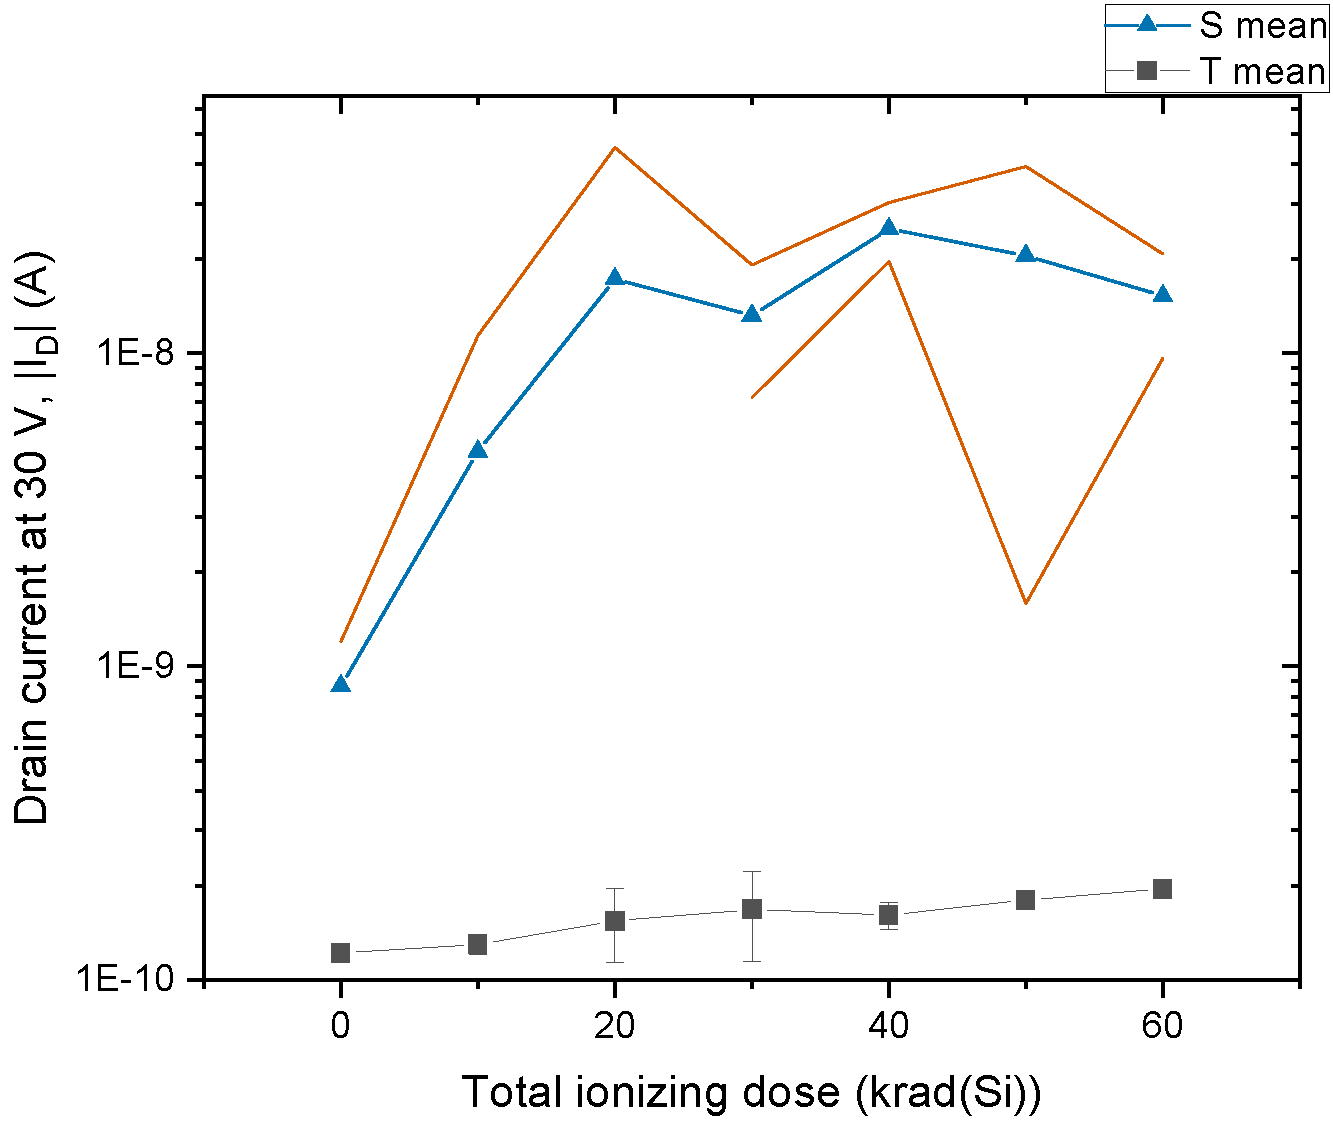
\includegraphics[keepaspectratio,alt={S/T组30 V漏电流随总剂量的变化}]{../03_figures/pdf/output_current_30v.pdf}}
\caption{S/T组30 V漏电流随总剂量的变化}
\end{figure}

达到 \(|I_D|=1\ \mu\)A 所需的漏极电压进一步反映曲线形状差异（图12）。S
组由 \(106.3\pm6.4\) V 降至 \(35.3\pm0.6\) V，配对变化为 \(-71.0\pm6.1\)
V；T 组则由 \(92.7\pm1.2\) V 升至 \(108.0\pm1.0\) V，配对变化为
\(15.3\pm0.6\)
V。两组方向相反，说明单一低压电流点不足以概括完整高压曲线。该阈值电压由
1 V 间隔采样点判定；曲线突变及合规限流起点也会影响其物理解释。

\begin{figure}
\centering
\pandocbounded{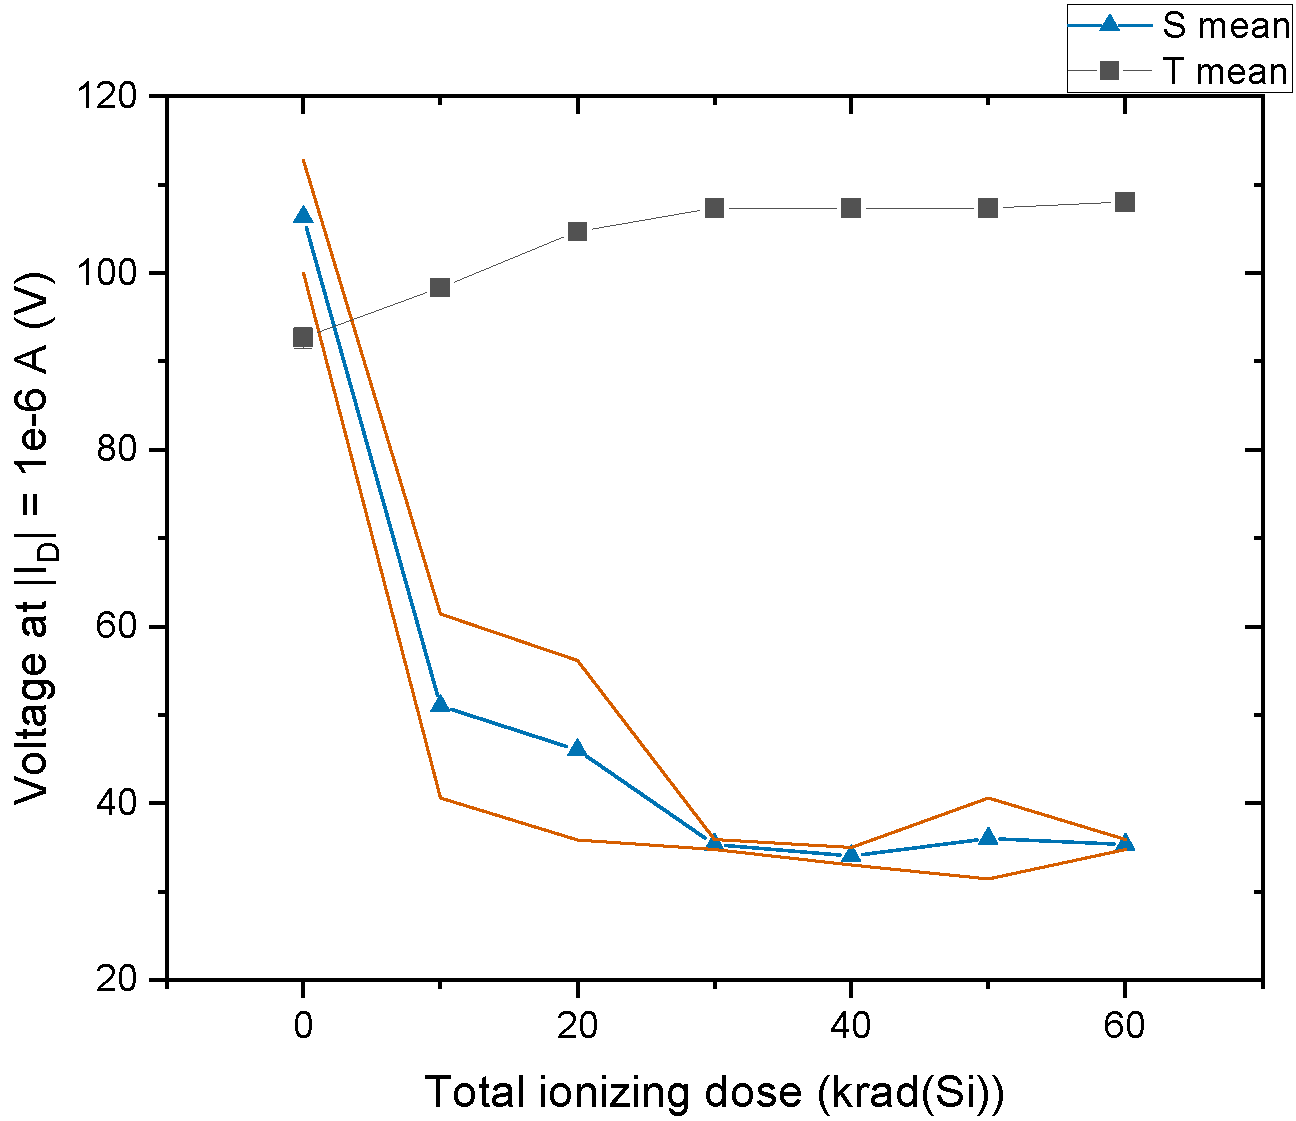
\includegraphics[keepaspectratio,alt={S/T组达到1 µA漏电流所需漏极电压随总剂量的变化}]{../03_figures/pdf/voltage_at_1ua.pdf}}
\caption{S/T组达到1 µA漏电流所需漏极电压随总剂量的变化}
\end{figure}

\textbf{统计归纳：} 转移参数表现出较平滑的剂量趋势，而 S
组输出漏电存在明显个体差异、非单调性和扫描历史依赖。故报告不把 150 V
电流、合规限流平台或某个单独器件的峰值解释为稳定的总剂量标志。

\section{4. S/T
两组纵向对比}\label{st-ux4e24ux7ec4ux7eb5ux5411ux5bf9ux6bd4}

在同一分析口径下，T 组在 60 krad(Si) 的负向阈值漂移比 S 组多约 3.85
V，亚阈值摆幅增量约为 S 组的 10.8 倍；两组峰值跨导相对降幅均约
60\%。另一方面，固定 \(V_{GS}=-20\) V、\(V_{DS}=30\) V 时，S
组漏电增加约 1.25 decade，而 T 组约 0.20 decade；达到 1 µA 的电压在 S
组降低、在 T 组升高。

\textbf{统计归纳而非因果结论：} 这些结果说明 S/T
两组的``转移特性退化模式''和``固定栅压输出响应''并不平行，不能用单一``耐辐照更好/更差''排序。阈值漂移、亚阈值摆幅、低场漏电和高压阈值电流分别描述不同的电学侧面。由于器件结构、材料、尺寸、工艺和封装属于商业保密信息，本报告只保留组标签层面的比较，不推测其内部设计差异。

\section{5.
连续加压扫描与恢复现象}\label{ux8fdeux7eedux52a0ux538bux626bux63cfux4e0eux6062ux590dux73b0ux8c61}

S 组在 20--60 krad(Si) 共保留 13 条 \texttt{scan\_no\textgreater{}1}
的后续输出扫描。它们分布不均：20 krad(Si) 1 条，30 和 40 krad(Si) 各 2
条，50 krad(Si) 3 条，60 krad(Si) 5
条；这些计数是复扫记录数，不是独立样本量。

\textbf{数据直接显示：} 在 30 V 处，全部 13
条后续扫描的漏电均低于同器件同剂量首次扫描，降低幅度为
70.65\%--96.19\%（图13）。按剂量观察，20 krad(Si) 的单条记录降低
95.90\%；30 krad(Si) 两条为 81.21\%--87.20\%；40 krad(Si) 两条为
93.22\%--94.05\%；50 krad(Si) 三条为 86.31\%--96.19\%；60 krad(Si)
五条为 70.65\%--79.14\%。例如 S3 在 50 krad(Si)
的第二、第三次扫描分别降低 95.29\% 和 96.19\%；S3 在 60 krad(Si)
的第二至第四次扫描分别降低 74.95\%、75.80\% 和
70.65\%，并未呈现严格随扫描次数单调增强的恢复。

\begin{figure}
\centering
\pandocbounded{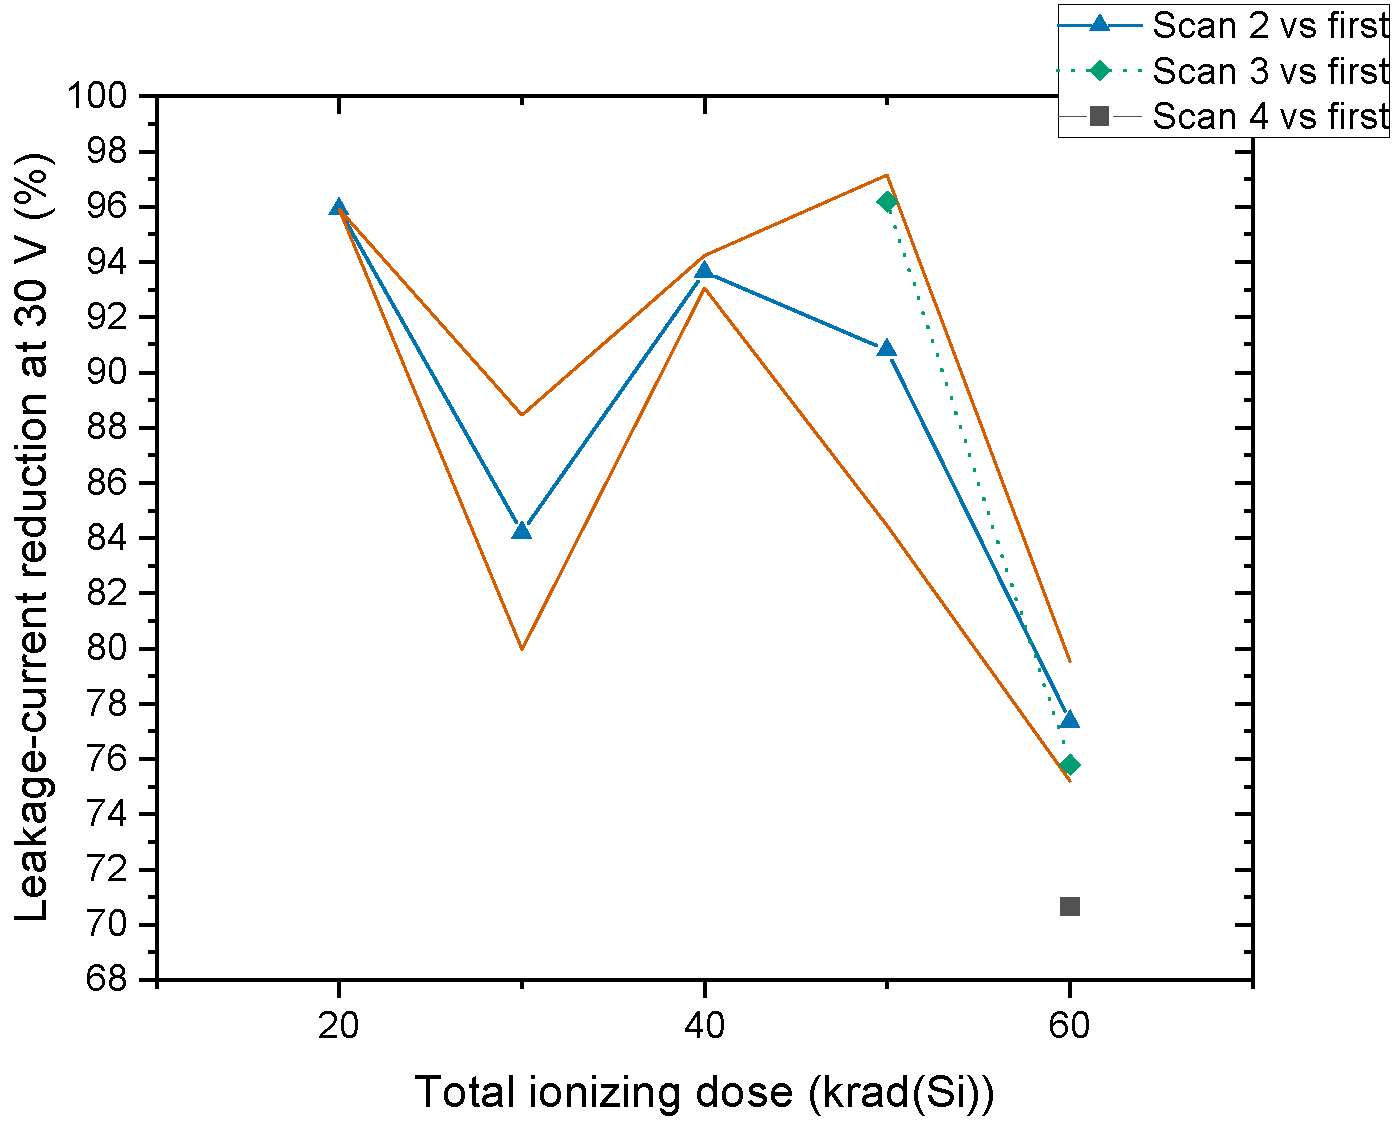
\includegraphics[keepaspectratio,alt={S组连续加压扫描后30 V漏电流相对首次扫描的降低}]{../03_figures/pdf/stress_recovery_30v.pdf}}
\caption{S组连续加压扫描后30 V漏电流相对首次扫描的降低}
\end{figure}

\textbf{统计归纳：} 后续扫描普遍降低 30 V
漏电，说明结果与加压/测量历史相关。各次连续扫描之间固定等待 20
min，使用同一台处于稳定状态的仪器，且无需切换量程，从而排除了等待时间不一致和量程切换作为主要差异来源。由于复扫器件和次数不平衡，这些百分比仍不能当作独立重复实验的总体均值，也不能与
n=3 的剂量主效应等同。

\section{6.
可能机制及替代解释}\label{ux53efux80fdux673aux5236ux53caux66ffux4ee3ux89e3ux91ca}

\textbf{文献支持：} MOS
结构的总电离剂量响应通常涉及氧化层内电子--空穴对产生、空穴俘获、界面态建立以及俘获电荷随时间、温度和电场发生退火或重新分布{[}1--4,6,7{]}。氧化层俘获电荷和界面陷阱均可影响阈值电压；界面态及近界面缺陷还会降低迁移率相关性能、增大亚阈值摆幅并提高噪声或漏电{[}1--5,8{]}。本实验观察到的负向阈值漂移、跨导下降和亚阈值摆幅恶化，与这些一般物理过程在现象层面相容。

\textbf{机制推断：} S
组连续高压扫描后漏电下降，可能与外加电场促进部分俘获载流子去俘获，或氧化层、近界面空间电荷重新分布有关。该解释与辐照后俘获电荷对电场、时间和温度敏感的文献认识相容{[}1--4{]}，但现有电学响应不能区分氧化层俘获电荷、界面态和边界陷阱的相对贡献{[}5{]}。这种机制分离不属于本报告的研究目标；未开展
C--V、charge pumping、低频噪声或温控退火，不作为待补实验。

\textbf{替代解释：} 连续扫描之间固定等待 20
min，测量使用同一台处于稳定状态的仪器，且无需切换量程，因此等待时间不一致和量程切换不作为主要解释。器件自热、探针或接触状态、前次高场测量改变后续初始条件、室温自然波动，以及低电流区零点或极性波动仍可能影响结果。质控记录显示，部分转移曲线在低电流区存在负
DrainI 点；本分析取 \(|I_D|\)
表示电流量级，不据符号变化推断物理机制。因此，``恢复''仅指观测到的扫描后漏电降低，不表示已建立因果关系。

\section{7.
适用范围与解释边界}\label{ux9002ux7528ux8303ux56f4ux4e0eux89e3ux91caux8fb9ux754c}

\begin{enumerate}
\def\labelenumi{\arabic{enumi}.}
\tightlist
\item
  每组仅 3
  个纵向器件。均值和标准差主要描述本批器件，不支持总体显著性或可靠性分布结论。
\item
  S/T
  仅为样品组标签。结构、材料、尺寸、工艺和封装按商业保密边界不予披露，也不由组间电学差异反推；这一边界不作为实验缺陷。
\item
  辐照在室温环境、20 V
  偏置及适当限流保护下进行。现有记录未提供剂量率和剂量学不确定度，因此即使每
  10 krad(Si) 的照射时间为 198
  s，也不自行换算或外推标准化剂量率{[}9,10{]}。
\item
  转移扫描范围随剂量改变，固定栅压电流的跨剂量比较受共同范围限制；亚阈值拟合窗口虽满足
  \(R^2\ge0.98\)，仍可能落在不同电压区段。
\item
  输出测试只有 \(V_{GS}=-20\) V 单栅压条件。高压端受约 10 mA
  合规限流影响，不能视为器件本征饱和特性，也不能解释为多 \(V_{GS}\)
  曲线族。
\item
  S 组复扫数据用于描述测量历史相关现象，不用于 S/T
  组间恢复能力比较。复扫次数不平衡，\texttt{-2/-3/-4}
  均为同器件后续扫描，不增加样本量。T
  组未设置对应复扫序列符合本报告的分析范围，不列为待补对照。
\item
  本报告旨在描述电学响应，而非分离微观缺陷机制。C--V、charge
  pumping、低频噪声和温控退火属于另一研究问题的实验手段，不是本报告的待补工作；相关机制仅作为候选解释{[}5{]}。
\end{enumerate}

\section{8. 结论}\label{ux7ed3ux8bba}

\begin{enumerate}
\def\labelenumi{\arabic{enumi}.}
\tightlist
\item
  \textbf{数据直接显示}，0--60 krad(Si) 累积辐照使 S、T
  两组阈值电压持续负向漂移，60 krad(Si) 时分别为 \(-6.120\pm0.045\) V 和
  \(-9.969\pm0.337\) V；峰值跨导均下降约 60\%。
\item
  \textbf{统计归纳}，三条器件轨迹的变化方向一致，但 T
  组亚阈值摆幅恶化更强，S 组固定 \(V_{GS}=-20\) V 下的 30 V
  漏电增幅和个体离散更大。不同指标给出的组间排序并不一致，因此不作单一优劣判定。
\item
  \textbf{数据直接显示}，S 组 13 条后续输出扫描的 30 V
  漏电相对首次扫描降低
  70.65\%--96.19\%，表明输出结果具有明显的加压/测量历史依赖。
\item
  \textbf{文献支持与机制推断}，氧化层俘获电荷、界面态以及场致去俘获或电荷重分布能够提供可能的物理框架。固定
  20 min
  扫描间隔、同一稳定仪器和无量程切换增强了恢复现象的可比性，但器件自热、接触状态和高场测量历史等替代解释仍不能完全排除，故不建立直接因果关系。
\end{enumerate}

\section{参考文献}\label{ux53c2ux8003ux6587ux732e}

{[}1{]} Oldham, T. R., \& McLean, F. B. Total ionizing dose effects in
MOS oxides and devices. \emph{IEEE Transactions on Nuclear Science},
2003, 50(3): 483--499. https://doi.org/10.1109/TNS.2003.812927

{[}2{]} Schwank, J. R., Shaneyfelt, M. R., Fleetwood, D. M., Felix, J.
A., Dodd, P. E., Paillet, P., \& Ferlet-Cavrois, V. Radiation effects in
MOS oxides. \emph{IEEE Transactions on Nuclear Science}, 2008, 55(4):
1833--1853. https://doi.org/10.1109/TNS.2008.2001040

{[}3{]} Fleetwood, D. M. Total ionizing dose effects in MOS and
low-dose-rate-sensitive linear-bipolar devices. \emph{IEEE Transactions
on Nuclear Science}, 2013, 60(3): 1706--1730.
https://doi.org/10.1109/TNS.2013.2259260

{[}4{]} Ma, T. P., \& Dressendorfer, P. V. (Eds.). \emph{Ionizing
Radiation Effects in MOS Devices and Circuits}. New York: John Wiley \&
Sons, 1989. ISBN 978-0-471-84893-6.

{[}5{]} McWhorter, P. J., \& Winokur, P. S. Simple technique for
separating the effects of interface traps and trapped-oxide charge in
metal-oxide-semiconductor transistors. \emph{Applied Physics Letters},
1986, 48(2): 133--135. https://doi.org/10.1063/1.96974

{[}6{]} Holmes-Siedle, A., \& Adams, L. \emph{Handbook of Radiation
Effects}, 2nd ed.~Oxford: Oxford University Press, 2002. ISBN
978-0-19-850733-8.

{[}7{]} Claeys, C., \& Simoen, E. \emph{Radiation Effects in Advanced
Semiconductor Materials and Devices}. Berlin: Springer, 2002.
https://doi.org/10.1007/978-3-662-04974-7

{[}8{]} Sze, S. M., \& Ng, K. K. \emph{Physics of Semiconductor
Devices}, 3rd ed.~Hoboken, NJ: John Wiley \& Sons, 2007.
https://doi.org/10.1002/0470068329

{[}9{]} ASTM International. \emph{ASTM F1892-12(2018), Standard Guide
for Ionizing Radiation (Total Dose) Effects Testing of Semiconductor
Devices}. West Conshohocken, PA: ASTM International, 2018.

{[}10{]} U.S. Department of Defense. \emph{MIL-STD-883, Test Method
1019: Ionizing Radiation (Total Dose) Test Procedure}. Washington, DC:
Department of Defense.

\end{document}
